% Fig. 2.14 / spec Fig A14 -- the median cuts the area under the density in
%   half.
% Source: mathstatch2.tex lines 2365-2404.
%
% Deviations from CH2_FIGURE_SPECS.md:
%
% 1. Curve.  The manuscript uses (45/4) x^3 e^{-1.7x} - 0.15, which does not
%    integrate to 1; per spec 1.6 the web uses Gamma(shape 4, rate 1.7),
%    f(x) = 1.3920167 x^3 e^{-1.7x}, plotted over 0:6.4 at y = 7.6cm.
%
% 2. Median.  The manuscript draws the boundary at 2, which is not the median
%    of the curve it draws.  Per spec 3.2 item 6 the web uses the true value
%    2.160036 (spec 1.6 gives 2.160035), where f = 0.356674.  With that
%    boundary the two areas really are 0.5 and 0.5; the right hand one as
%    drawn is 0.494620, the missing 0.005380 being the tail past 6.4.
%
% 3. Shading path.  The manuscript's \fill starts at (2.6,0), a point with no
%    relation to the boundary, which leaves a notch along the left edge of the
%    shaded block (spec 3.2 item 4).  The path here follows spec 1.6: along
%    the axis from 0 to the boundary, up to the curve, back along the curve.
%
% 4. Type size of the two 1/2 labels.  The manuscript sets them \small.  At
%    \small the digits of an inline fraction fall to script size of 9pt, i.e.
%    7pt, which shows at 11.9px on a 350px phone and breaks the 12px floor of
%    spec 1.3.  They are set at \normalsize instead, which spec 1.3 permits
%    (\small is a floor, not a requirement).
%
% 5. The manuscript puts the x label at (6.5,0.15) while the axis stops at
%    6.2.  Per spec 1.3 the label goes at the end of the axis instead.
%
% 6. \DeclareMathSizes{10}{10}{9}{8}, as in the rest of this group; not the
%    site-wide \sssig change that ruling 21 defers.  Native size
%    206.796 x 110.284 pt, drawing range 7.15cm wide, inside the 9.0cm cap; the
%    box is shared with quantile-intuition.tex and quartiles-equal-areas.tex,
%    which draw the same curve at the same scale.  At the 350px phone width
%    that gives 16.9px for 10pt text, 15.2px for 9pt scripts and 13.5px for
%    8pt scriptscripts; at 620px 29.9 / 26.9 / 23.9px.
%
% The density is written as 1.3920167 (x e^{-0.56666667x})^3 because pgfmath
% cannot hold e^{1.7x} at the right hand end of the range.
\documentclass[tikz,border=2pt]{standalone}
\usepackage{amsmath}
\usepackage{amssymb}
\usepackage{xcolor}
\usetikzlibrary{arrows.meta}
\newcommand{\sssig}{\scriptscriptstyle}
\DeclareMathSizes{10}{10}{9}{8}

\definecolor{journalink}{HTML}{1F1C18}
\definecolor{journalmuted}{HTML}{8A7F72}
\definecolor{journalaccent}{HTML}{9C2D2D}

\begin{document}
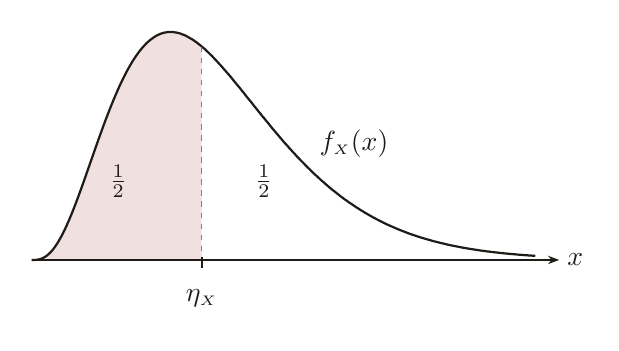
\begin{tikzpicture}[
  x=1cm,
  y=7.6cm,
  every node/.style={font=\normalsize, journalink},
  axis/.style={journalink, line width=0.8pt, -{Stealth[length=4pt]}},
  tick/.style={journalink, line width=0.8pt},
  curve/.style={journalink, line width=0.8pt},
  guide/.style={journalmuted, line width=0.5pt, dash pattern=on 2pt off 2pt},
  region/.style={journalaccent, fill opacity=0.15}
]
  % ---- bounding box shared with the other two Gamma(4,1.7) figures ------
  \path (-0.05cm,-0.80cm) rectangle (7.10cm,2.95cm);

  % ---- the left half of the area ---------------------------------------
  \fill[region]
    (0,0) -- (2.160036,0) -- (2.160036,0.356674)
    -- plot[domain=2.160036:0, samples=200, smooth]
       (\x,{1.3920167*pow(\x*exp(-0.56666667*\x),3)}) -- cycle;

  % ---- density curve: Gamma(4, 1.7) ------------------------------------
  \draw[curve] plot[domain=0:6.4, samples=300, smooth]
    (\x,{1.3920167*pow(\x*exp(-0.56666667*\x),3)});

  % ---- x axis ----------------------------------------------------------
  \draw[axis] (0,0) -- (6.7,0);
  \node[anchor=west, inner sep=2.8pt] at (6.7,0) {$x$};

  % ---- the median ------------------------------------------------------
  \draw[guide] (2.160036,0.356674) -- (2.160036,0);
  \draw[tick] ([yshift=0.035cm]2.160036,0) -- ([yshift=-0.106cm]2.160036,0);
  \node[anchor=north] at ([yshift=-0.25cm]2.160036,0) {$\eta_{\sssig X}$};

  % ---- one half of the area on either side ------------------------------
  \node[inner sep=0pt] at ([yshift=1.00cm]1.100,0) {$\frac{1}{2}$};
  \node[inner sep=0pt] at ([yshift=1.00cm]2.950,0) {$\frac{1}{2}$};

  % ---- curve label -----------------------------------------------------
  \node[anchor=south west, inner sep=0pt] at ([yshift=1.30cm]3.65,0)
    {$f_{\sssig X}(x)$};
\end{tikzpicture}
\end{document}
